\section{Aplicación web}

La siguiente Figura \ref{fig:procesoApp} muestra las etapas que se llevarán a cabo por parte de la aplicación web.
\begin{figure}[ht]
\centering
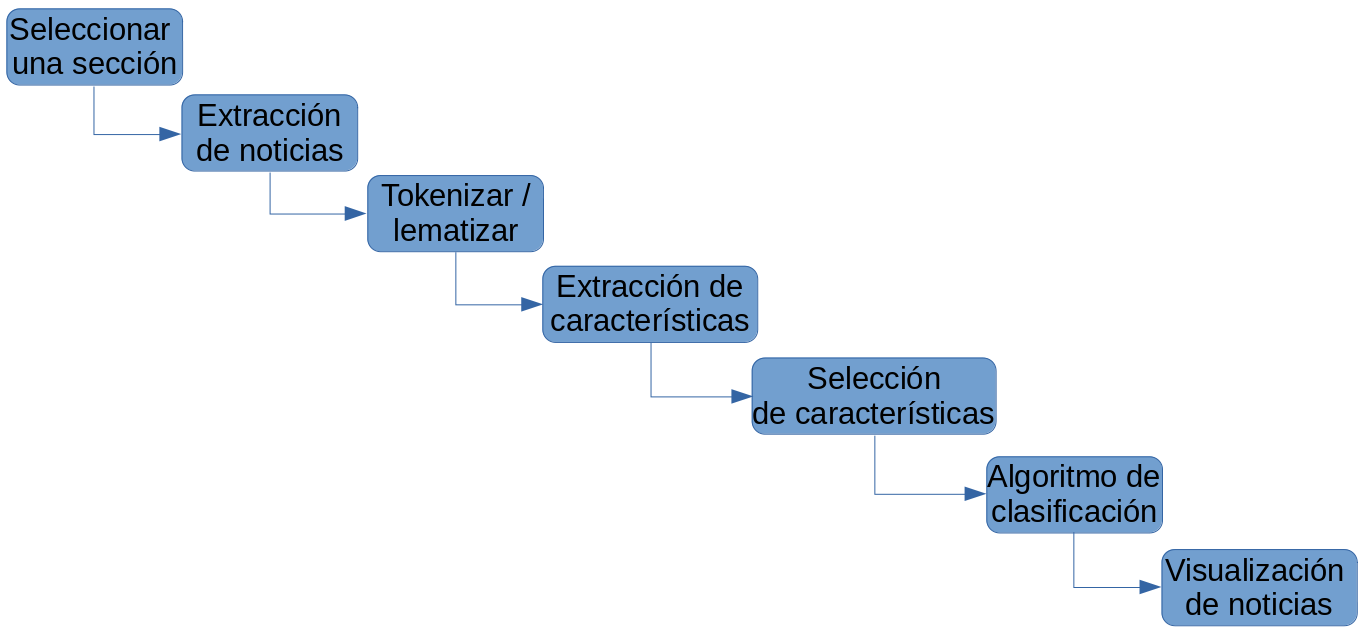
\includegraphics[scale=0.3]{imagenes/Capitulo5/procesoAplicacionWeb.png}
\caption{Etapas de la aplicación web}
\label{fig:procesoApp}
\end{figure}

\subsection{Tecnologías utilizadas}
A continuación se describen las tecnologías y librerías que han sido utilizadas durante el desarrollo del sistema Web.

\subsubsection{JavaServer Faces}
JavaServer Faces es una tecnología utilizada para desarrolladar aplicaciones web la cual permite el desarrollo de interfaces de usuario.

\subsubsection{}

\subsection{Proceso de recolección}
La aplicación web tiene como objetivo recolectar y clasificar noticias, por ello la primera parte que se debe realizar es la recolección de noticias, como se mencionó en el apartado 5.1 se han definido los sitios web de donde las noticias serán recolectadas, la información recuperada śerá:

\begin{itemize}
	\item URL de la noticia
	\item Título
	\item Fecha
	\item Autor
	\item Descripción \footnote{Existen sitios web, donde no todas las noticias cuentan con una descripción}
	\item Noticia
\end{itemize}

Cabe destacar que en este punto, ya no será necesario extraer el nombre de la sección a la cual pertenece la noticia, dado que el clasificador lo realizará de manera automática.\\

\subsection{Proceso de clasificación}
Una vez que las noticias han sido recolectadas, deberán pasar por dos pasos fundamentales, como primer paso la noticia debe ser tokenizada y lematizada, posteriormente se deben extraer las características de cada noticia, esto permitirá al algoritmo seleccionado obtener un mejor resultado en el momento de realizar la clasificación.

\subsection{Frontend}

Para la realización de la aplicación web es necesario utilizar herramientas que nos permitan visualizar las noticias clasificadas, por ello las interfaces de usuario se desarrollarón en utilizando el Framework Java Server Faces.

La Figura \ref{fig:PantallaInicio} muestra la vista que tendrá el usuario al ingresar a la aplicación web

\begin{figure}[ht]
\centering

\includegraphics[scale=0.3]{imagenes/Capitulo5/inicio.png}
\caption{Pantalla de Inicio.}
\label{fig:PantallaInicio}
\end{figure}

El usuario tiene la posibilidad de elegir la sección de la cual desee visualizar noticias. La Figura \ref{fig:loading} muestra la vista que tendrá el usuario dar click en una sección.

\begin{figure}[ht]
\centering
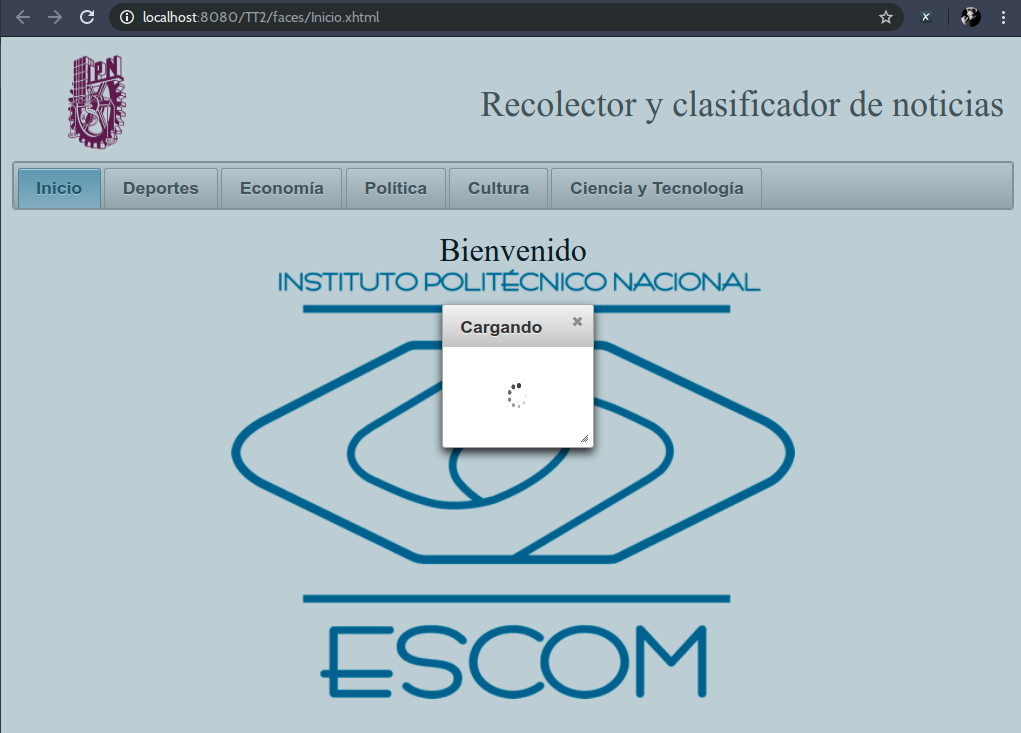
\includegraphics[scale=0.3]{imagenes/Capitulo5/cargando.png}
\caption{Pantalla de espera}
\label{fig:loading}
\end{figure}

Una vez finalizado el proceso de recolección de noticias


